%!TEX root = main.tex

%\paco{Ahmed is going to work on a pre-version of this by adding all the graphs}
In this section we analyze the process that participants use to evaluate translation. We focus on three different aspects. First, we use \eye data to observe in which areas do participants spend most of their time. Next, we analyze the time that participants take to complete the evaluation. Finally, we analyze the scores given by the participants, and their consistency.

\vspace{5pt}
\subsection{How Long Does it Take?}
\vspace{5pt}

One important aspect to take into account is the time at which annotations can be collected \cite{callisonburch-EtAl:2007:WMT}. To discount the time a participant spends idle (be either by fatigue, distraction, etc.), here we analyze only the \emph{focused} time, i.e. the amount of time a participant gaze is focused in \emph{areas of interest}.
\\
 In our experiments, we observed that on average annotations take $26.06$  seconds to be collected, which is in line with the measurements reported by \newcite{callisonburch-EtAl:2007:WMT}. In Table~\ref{tab:time-length}, we further break down the task durations by: \Ni type of evaluator (i.e. \mono and \bil), \Nii \gamet (i.e. \src, \srctgt, and \tgt); and  \Niii the length of the source sentence (i.e. \lshort, \lmid, \llong).


\begin{table}[htb]
\vspace{5pt}

\small
\begin{tabular}{rllrrrr}
  \toprule
 & scnr. & usr\_type & \llong & \textit{med} & \lshort & avg \\ 
  \midrule
1 & src & biling & 36.89 & 24.54 & 17.92 & 26.46 \\ 
  2 & src & mono & 44.11 & 28.58 & 19.17 & 30.55 \\ 
  3 & src+tgt & biling & 40.16 & 23.99 & 15.46 & 26.59 \\ 
  4 & src+tgt & mono & 46.76 & 29.69 & 21.63 & 32.71 \\ 
  5 & tgt & biling & 26.41 & 15.03 & 10.54 & {\bf 17.28} \\ 
  6 & tgt & mono & 35.90 & 19.41 & 12.69 & 22.77 \\ 
   \bottomrule
\end{tabular}
\caption{\label{tab:time-length}Average task duration time (in seconds) according to type of setup, type of evaluator and source sentence length.}
\vspace{5pt}

\end{table}


The first observation to make is that \bil evaluators are consistently faster than \mono evaluators in evaluation. This is true even in the \tgt condition, where both evaluators can leverage the same amount of information (i.e. both are fluent in English). %\paco{ I DONT KNOW IF THIS SHOULD GO HERE OR LATER.} 
This can have two possible explanations: \Ni \bil evaluators develop \emph{internal} rules that allow them to perform the task faster, and \Nii since the order of the conditions was fixed (i.e evaluators performed first the \src tasks, then the \srctgt tasks and lastly the \tgt tasks), this could mean that the \bil evaluators got \emph{more efficient} sooner, just because the \src task wasn't noise to them. However, we show later that \Ni is more plausible.

The second observation to make is that evaluators tend to take longer to evaluate scenarios with more sources of information available. This is true for \mono if we analyze the results either by \gamet or by source length\footnote{Longer source sentences have more words.}. Surprisingly, \mono participants in the \src condition perform the task $7\%$ faster than in the \srctgt condition, which leads to hypothesize that the more information is in the screen, the longer the task will take, even if the information is not particularly useful for the task completion. On the other hand \bil take the least time when evaluating \tgt scenario.\\ %\irina{This observation has been confirmed by the final feedback provided by the participants (see Section 2.6)}.

To measure the significance of our observations, we fitted a random intercepts model  and analyzed the relationship between task duration time, length of the sentences, type of evaluator and type of scenario while taking into account the variability between evaluators. Therefore, as fixed effects, we had the length of the sentences, the type of evaluator (\bil and \mono) and the \gamet into the model. We also included the interaction between the type of evaluator and the length of the sentences. As random effects, we had intercepts for each of the 20 evaluators. P-values were obtained by likelihood ratio tests of the full model with the effect in question against the model without the effect in question. 
\vspace{5pt}

In general, the effect of \gamet is highly significant ($\chi^2_{2}=121.71$, $p=2.2e^{-16}$), and for long sentences the \tgt scenario is $8.52$ and $9.6$ seconds faster than the \src and \srctgt scenarios, respectively. The effect of the type of evaluator is also significant  ($\chi^2_{3}=7.45$, $p=0.05$), and on average \bil are faster than \mono by $7.76$ seconds for long sentences. These results were obtained using R \cite{R:2015} and lme4 \cite{LM4:2015}, following \newcite{DBLP:journals/corr/Winter13}.


%Analyzing evaluator's speed from Figures ~\ref{fig:TimeScoremax} and ~\ref{fig:TimeScoremin}, shows that bilingual evaluators are relatively faster in completing tasks for both max and min types. Bilingual mean, max is (27.51,64.91) versus (33.78,121.65) for the Monolinguals. Monolingual evaluator's speed varies widely. Scoring ``max'' category takes more time for both evaluator types.
%Here we evaluate how evaluators's speed is, and how does it affect results if any.
%\begin{figure}[ht]
%\centering
%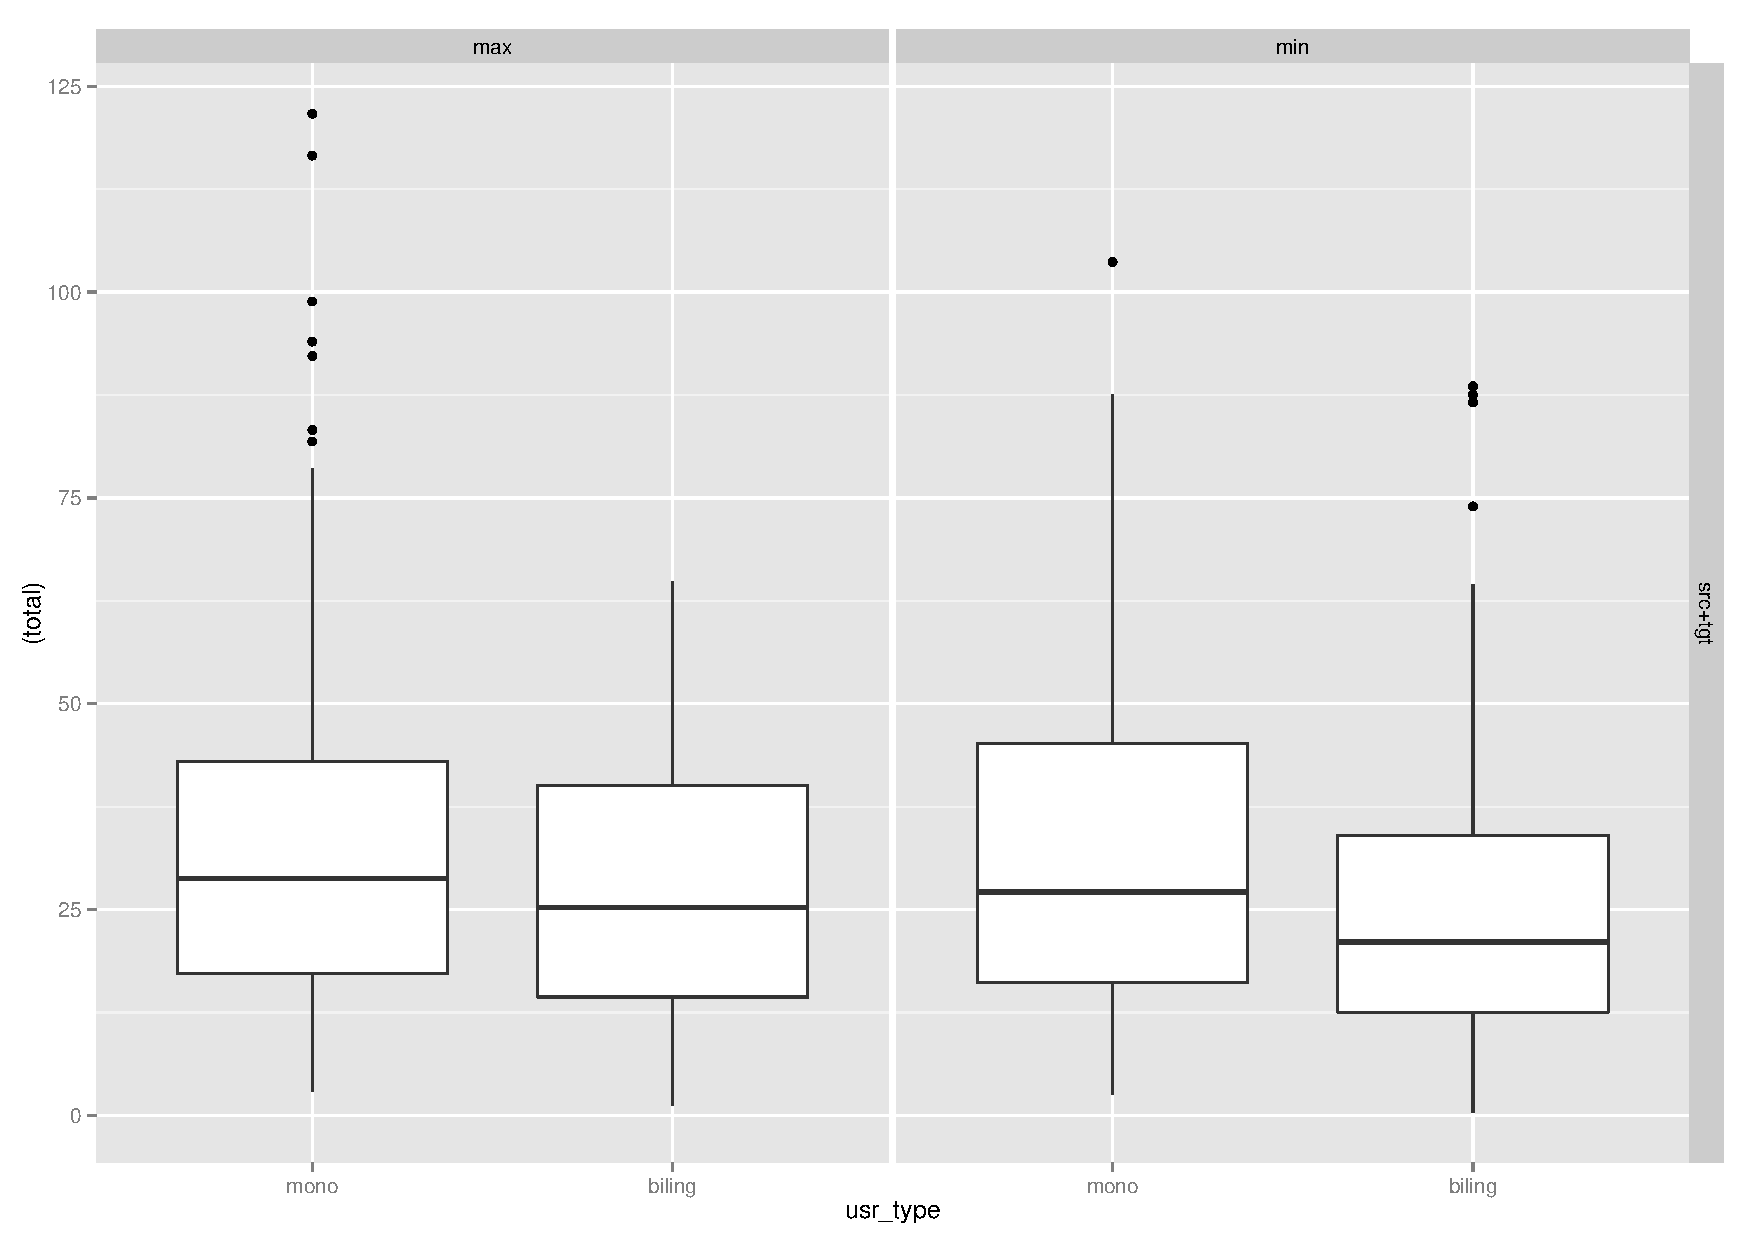
\includegraphics[scale=0.265]{data/time_srctgt.pdf}
%\caption{Users time in src+tgt scenario}
%\label{fig:TimeScoremax}
%\end{figure}


\vspace{10pt}
\subsection{Where Do Evaluators Look?}
\vspace{5pt}

The \eye data allowed us to analyze the behavior of the evaluators across different conditions. In particular, we focused in the \emph{dwell} time, i.e. the amount of time an evaluator is looking at a particular \emph{area of interest} in the screen. In Table~\ref{tab:aoi}, we present the proportional \emph{dwell} time (out of the \emph{focused} time) that the evaluators spent in the different areas of the screen: \Ni translation, \Nii source (with previous and next context), \Niii reference (with previous and next context), \Niv and the sum of the source and reference times.\\



\begin{table}[ht]
\centering
\small
\begin{tabular}{rllrrrr}
  \toprule
 & scnr. & usr\_type & tra & ref & src & src+ref \\ 
  \midrule
1 & src & mono & 0.18 & - & 0.82 & 0.82 \\ 
  2 & src & biling & 0.12 & - & 0.88 & 0.88 \\ 
  3 & src+tgt & mono & 0.13 & 0.24 & 0.63 & 0.87 \\ 
  4 & src+tgt & biling & 0.07 & 0.16 & 0.78 & 0.93 \\ 
  5 & tgt & mono & 0.26 & 0.74 & - & 0.74 \\ 
  6 & tgt & biling & 0.19 & 0.81 & - & 0.81 \\ 
   \bottomrule
\end{tabular}
\caption{\label{tab:aoi} Proportional time spent by evaluators while focusing in different regions of the screen: translation (trans), reference and its context (ref), source and its context (src), and the aggregate of src and ref.}
\end{table}

%\\
From the table, the main observation is that evaluators spend most of their time looking at regions other than the translation (src+ref). This supports the hypothesis that evaluators try to understand the source and reference before making a judgment about the translation. However, there are some peculiarities worth noting. First, \bil participants spend less time reading the translation than their \mono counterparts. %This is particularly noticeable in the \srctgt condition, where \bil evaluators spend about $78\%$ of their time reading the source(s), and only $7\%$ of their time reading the translation. 
\\
\pagebreak
\vspace{10pt}

For example, this means that on average, in the \tgt condition, a \bil evaluator would spend  $5$ ($0.19*26.41$) seconds\footnote{This time does not need to be continuously spent on the same region. For example, a evaluator might analyze a first portion of a translation, then move back to the reference, and then return to the translation.} focused on a \llong translation while a \mono evaluator would spend $9.3$ ($0.26*35.9$) seconds, that is almost \underline{double} the time. In contrast, the difference times both \bil and \mono evaluators would spend reading the reference is only a factor of $1.2$ ($21.3$ and $26.6$ seconds, respectively). This tells that \bil are faster (mostly) because they spend \emph{less} time reading the translation.

Another interesting observation is that \mono spend a sizable proportion of their time reading the source (which they supposedly \emph{do not} understand), even in the \srctgt scenario. This suggests that \mono evaluators develop \emph{rules-of-thumb} to analyze the source, even if it is a foreign language (e.g. translation of named entities, numbers, dates). This can be an artifact of the relatedness between English and Spanish, or an priming effect induced by the order in which the tasks were done (i.e by asking \mono evaluators to score \src tasks first, we forced them into developing this behavior). The analysis of such phenomena, while interesting, is beyond the scope of this paper.

Finally, if we look across conditions, we observe that evaluators spend a larger proportion of their time evaluating the translation in the \tgt condition than in the \src and \srctgt conditions. Yet, when we calculate the expected focused time in the translation region for each condition (across different lengths and evaluator types), we obtain $4.48$, $4.35$ and $2.85$ seconds for each condition, respectively. \\


This tells us that having more information on the screen (the case of \srctgt) decreases the total amount of time spent reading the translation. In other words, if a evaluator has more sources of information to evaluate a translation, s/he'll spend more time performing the task, but less time evaluating the translation itself. 

% The data collected showed that background of evaluators has an impact on translation. While both evaluators type (mono- and bi-linguals) uses all the information available to them as shown in Figure ~\ref{fig:evaluatorsregionsmin} and ~\ref{fig:evaluatorsregionsmax}; both they tend to use the information is different way depending on the game and quality. In the next sections, we will dive deeper on the various aspects of these differences trying to answer our research questions and reveal key information about the evaluation process. 
% \begin{figure}[ht]
% \centering
% 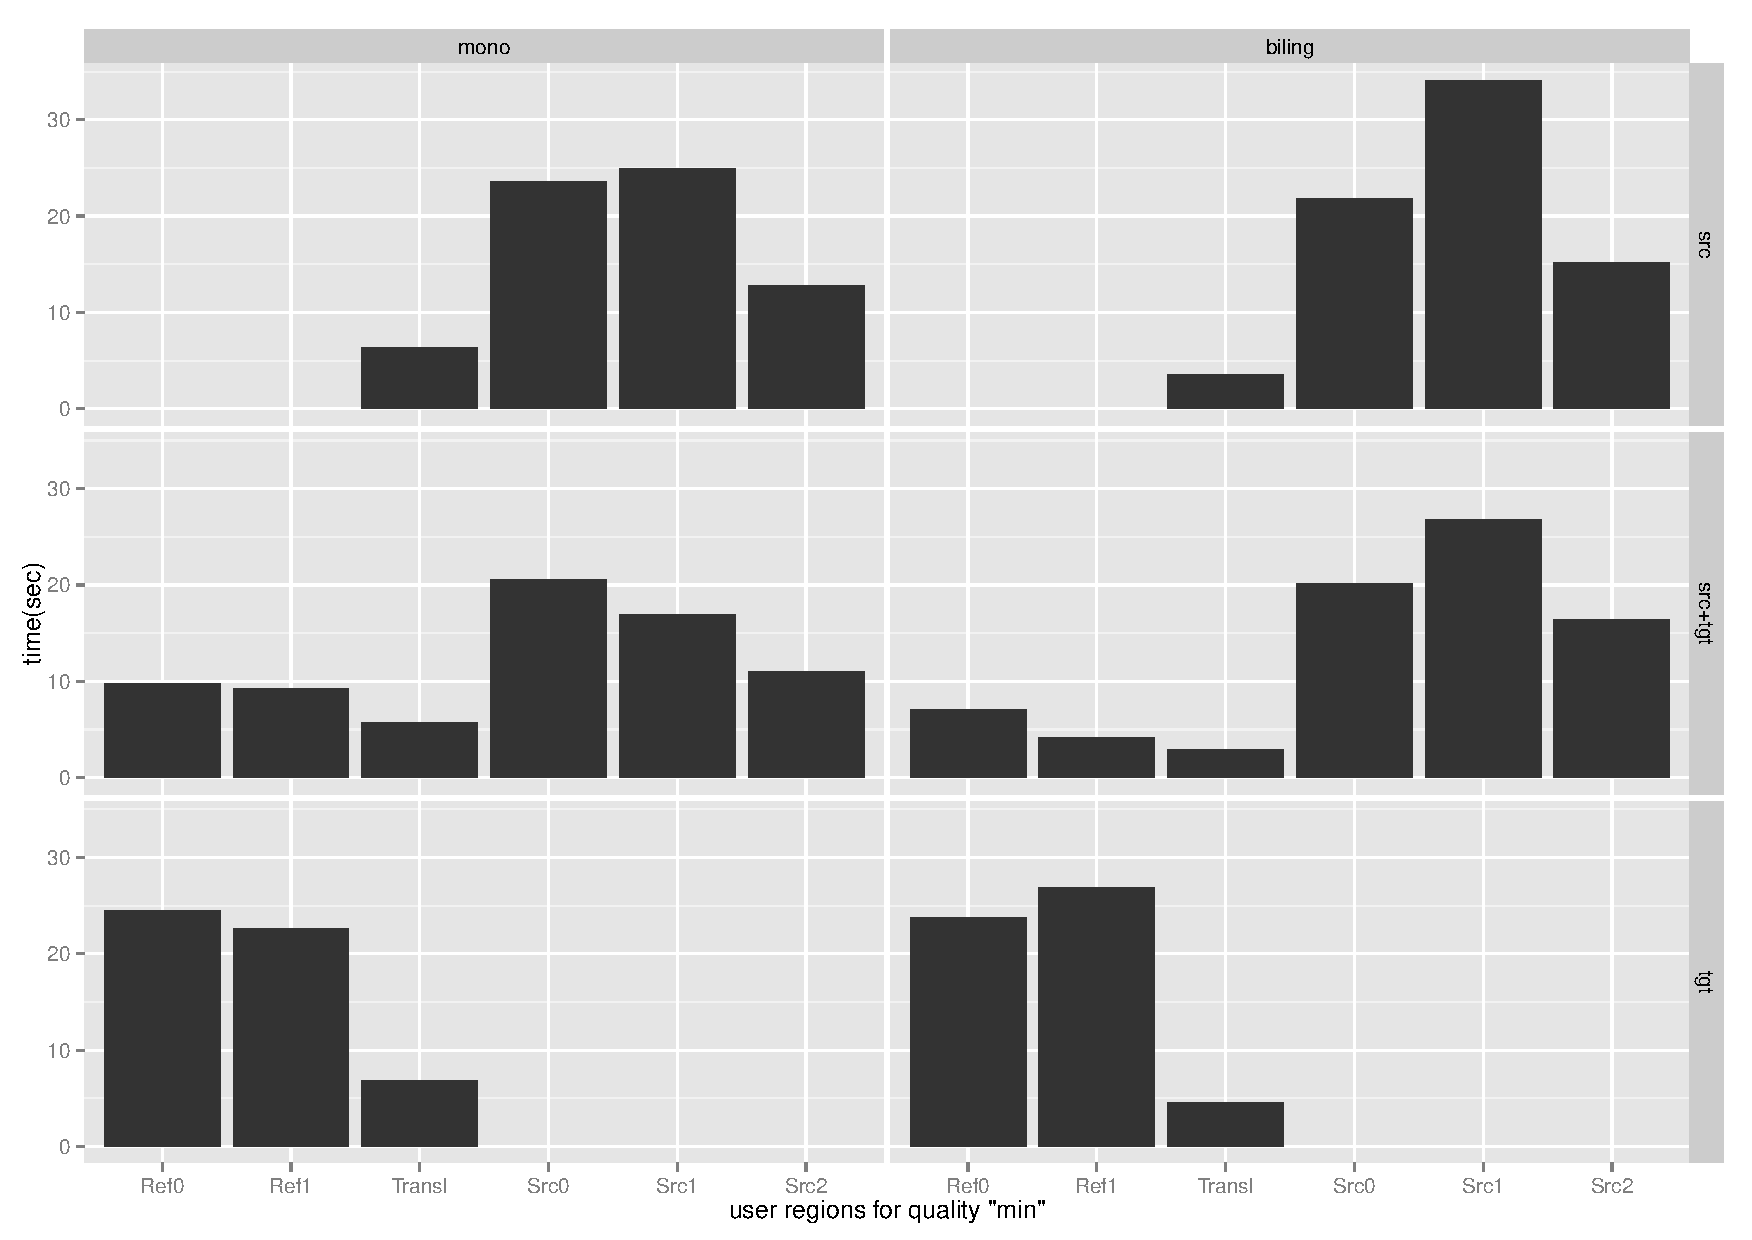
\includegraphics[scale=0.275]{data/Users_regions_min.pdf}
% \caption{Users time in regions while scoring ``min'' category.}
% \label{fig:evaluatorsregionsmin}
% \end{figure}
% \begin{figure}[ht]
% \centering
% 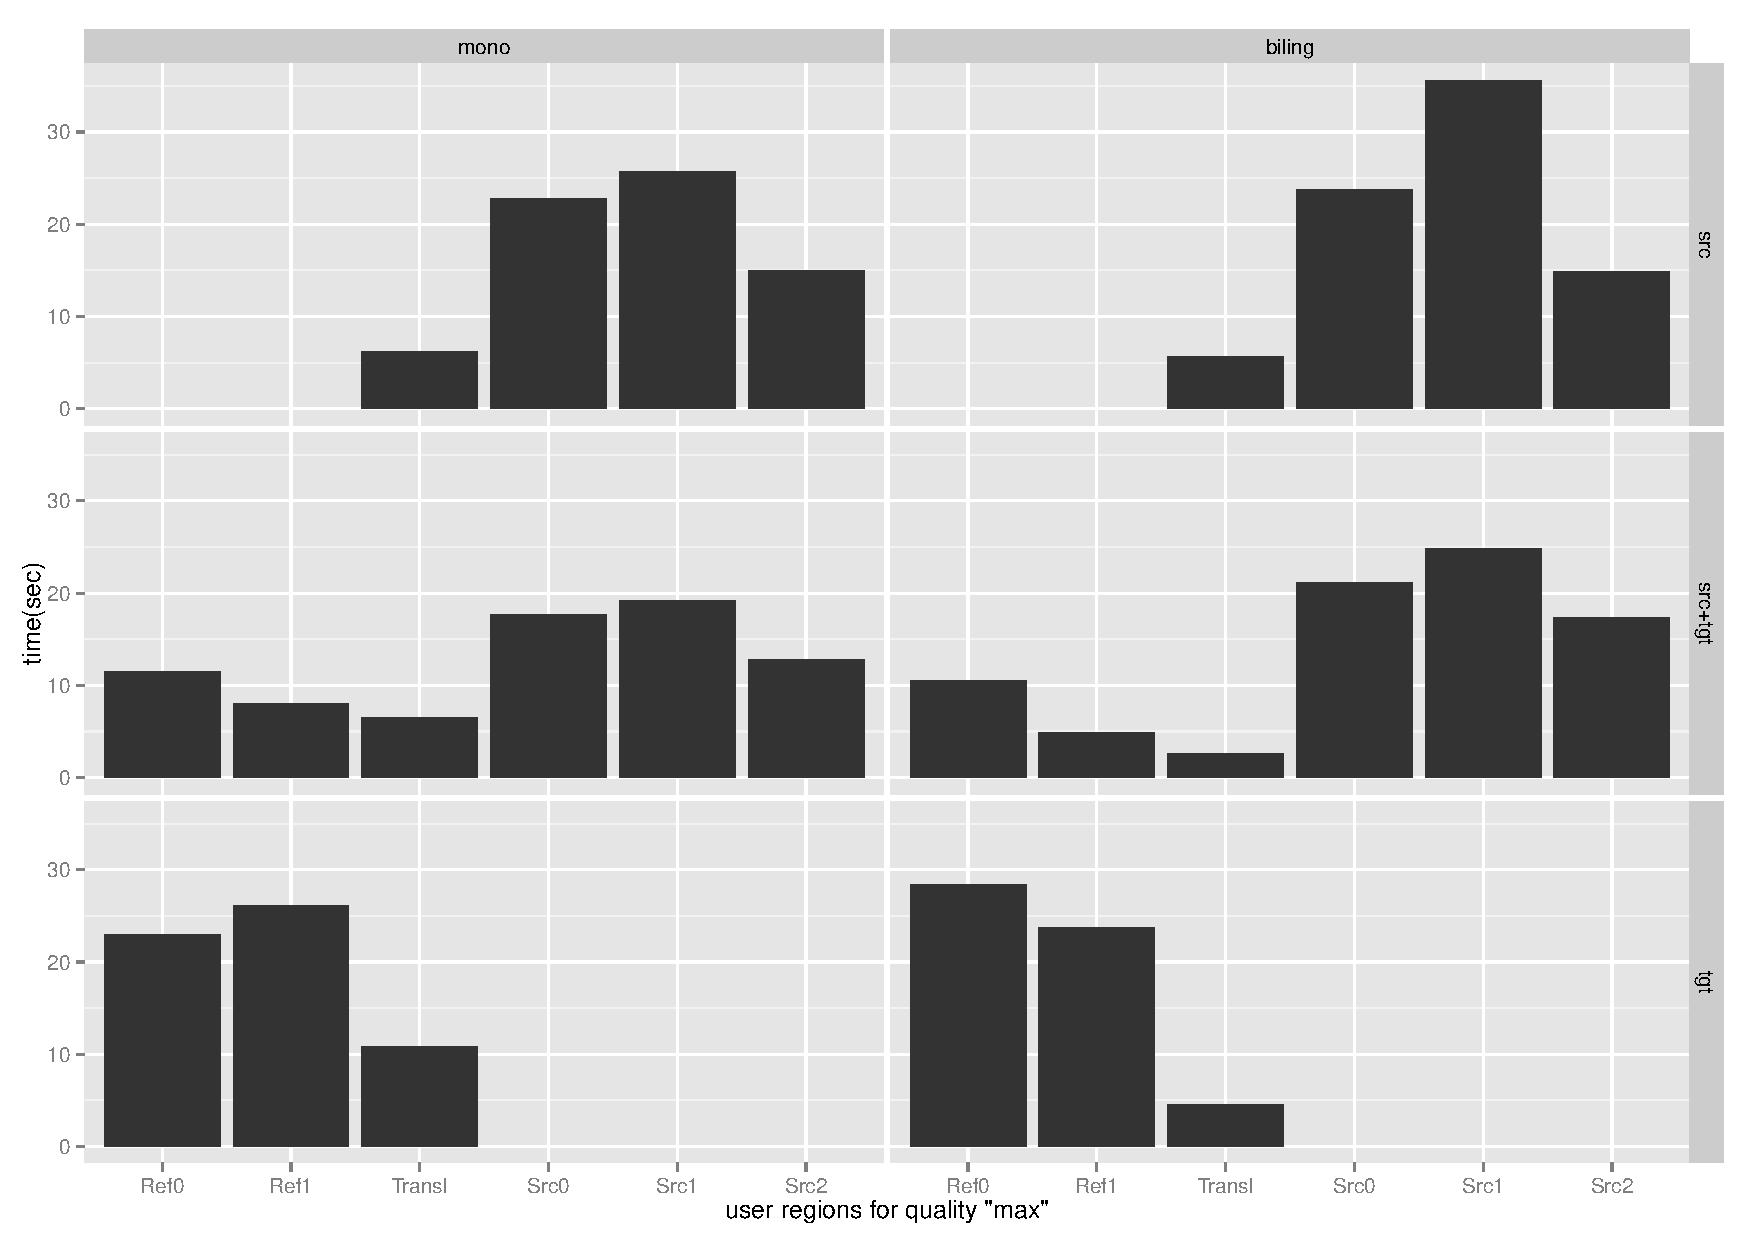
\includegraphics[scale=0.275]{data/Users_regions_max.pdf}
% \caption{Users time in regions while scoring ``max'' category.}
% \label{fig:evaluatorsregionsmax}
% \end{figure}

\vspace{3pt}
\subsection{Score Consistency} 
Another important aspect to take into account is how consistent are the scores provided by different evaluators, and how this consistency varies depending on the type of evaluator, and the \gamet that is used. Unlike other studies where categorical and ordinal scores are produced, here each annotation generates a score in a continuous scale\footnote{Actually it is an ordinal scale from 0-100, but for practical purposes we treat it as continuous}. Thus, using the standard inter-annotator agreement is impractical. Instead, we evaluate \emph{consistency} as the standard deviation of scores for each translation with respect to a class or group average (i.e. \mono or \bil). This quantity gives us an idea of how much variation there is in the score for a specific translation across different groups of evaluators. To be able to compare across evaluators, we  normalized their individual scores to a 0-1 range using \emph{minmax}. Then, computed the consistency as follows:

\begin{equation}\label{eq:1}
\sigma_c^2 =   \frac{1}{N_c}\sum_{i \in T} \sum_{j\in C} (\tilde x_{ij} - \bar{\tilde x}_{ic})^2
\end{equation}

\noindent where $\tilde x_{ij}$ is the \emph{normalized} score of translation $i$ by an evaluator $j$ who belongs to class $c$ (e.g. \mono), and $\bar{\tilde x}_{ic}$ is the average score given to translation $i$ by evaluators in class $c$, and $N_c$ is the total number of translations scored by evaluators in class $c$. \\

In Table~\ref{tab:consistency} we present the consistency measurements for \mono and \bil evaluators across the different conditions. 

 %We measured the consistency between evaluators \emph{cost}, group \emph{cost\_group} and versus original scores \emph{hum\_cost} as shown in Figure~\ref{fig:evaluatorconsistency}. Monolinguals shows that they are more consistent (\emph{lower cost}) cross all \gamet{s}. 


\begin{table}[ht]
\centering
\small
\begin{tabular}{rllr}%}
  \toprule
 & scnr. & usr\_type & $\sigma_c$  \\%& $\tau_c$ \\ 
  \midrule
1 & src & mono & 15.14 \\%& 28.79 \\ 
  2 & src & biling & 16.17 \\%& 29.74 \\ 
  3 & src+tgt & mono & 14.88 \\%& 27.04 \\ 
  4 & src+tgt & biling & 15.96 \\%& 26.22 \\ 
  5 & tgt & mono & {\bf 14.13} \\%& {\bf 24.73} \\ 
  6 & tgt & biling & 16.81 \\%& 27.62 \\ 
   \bottomrule
\end{tabular}
\caption{\label{tab:consistency}Consistency scores: standard deviation with respect to the class average ($\sigma_c$) %and with respect to the human ranking scores ($\tau_c$) 
for the scores produced by different types of evaluators across different conditions. Lower scores means higher consistency. Each measure is calculated over $N=200$ points.}
\vspace{-10pt}
\end{table}

First note that \mono evaluators are more consistent within their group ($\sigma_c$) than the \bil evaluators. This observation holds true across all the different scenarios. Note also that \mono evaluators are the \emph{most} consistent in the \tgt condition.  We hypothesize that this is due to the longer times spent analyzing the translation in comparison to \bil evaluators. But also, we think this is related to the simplicity of the task. There is less information to analyze. On the other hand \bil, have a larger variation, which can be attributed to the heterogeneity of \emph{rules of thumb} that the evaluators develop from looking at the source.
%Also note that \mono users in the \tgt have the least deviation from the \emph{corrected} human ranking scores, which tells us that the user scores are more in agreement with the rankings provided in the WMT12 tasks for the same translations.
Finally, note how \bil have a problem of consistency with the \tgt task. Without more fine-grained information, we can only hypothesize that this is due to the lack of familiarity with the scenario. Before performing tasks in the \tgt scenario, they were relying primarily on the source to evaluate.% This can be due to the %Here we tell how users are consistent with each other and with the ranking/provided scores

%\begin{figure}[ht]
%\centering
%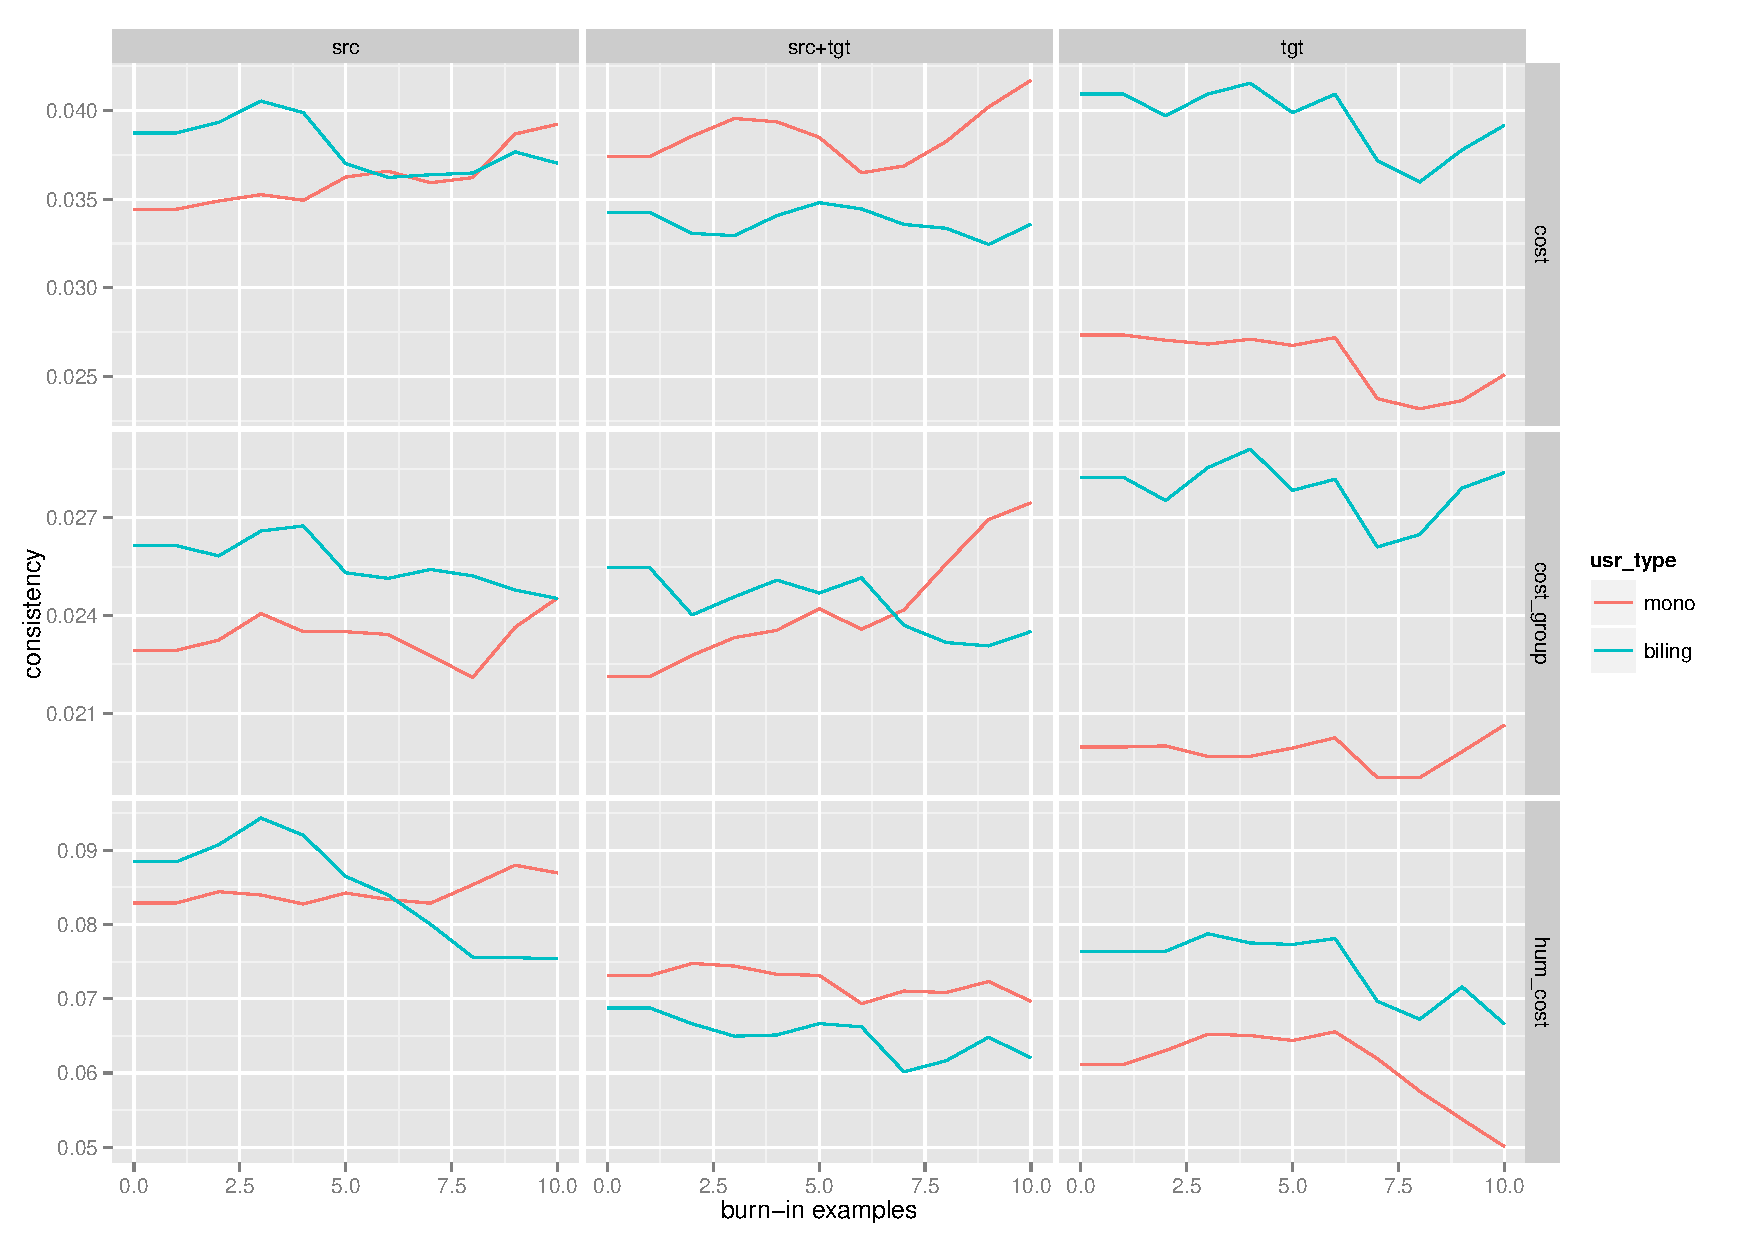
\includegraphics[scale=0.29]{data/consistency.pdf}
%\caption{Users consistency in various scenarios}
%\label{fig:userconsistency}
%\end{figure}

\subsection{Summary of Observations}
We have observed that there are differences in how translations are evaluated according to the type of evaluator, and the scenario. In summary, the observations are:
\begin{itemize}
\item The \bil evaluators perform the tasks faster than the \mono. They also spend less time evaluating the translation.
\item The \mono evaluators are slower, but more consistent in the scores they provide. %When only the source information is displayed, \mono evaluators still 
\item The more information is displayed in the screen, it will take to longer to complete the evaluation, even though, less time will be spent actually evaluating the translation. Displaying more information also correlates with lower consistency between evaluators.
\end{itemize}

% \subsection{User Behavior}
% %Here we discuss how users evaluate. 
% Figures ~\ref{fig:behavbilgmax} and  ~\ref{fig:behavmonomax} present the users behavior while evaluating sentences from ``max'' category. The circles size represents the proportional time spent in the area while the directed arcs width reflect the frequency of the transition between the connected regions. From the figures, we can note that the bilingual users tend to spend more time between source -See Figure ~\ref{fig:behavbilgmax}- regions when compared to monolinguals. Monolinguals move back and forth between source and reference more frequently when scoring ``max'' category as shows Figure ~\ref{fig:behavmonomax}.
% %What are the differences across regions in the layout
% \begin{figure}[ht]
% \centering
% 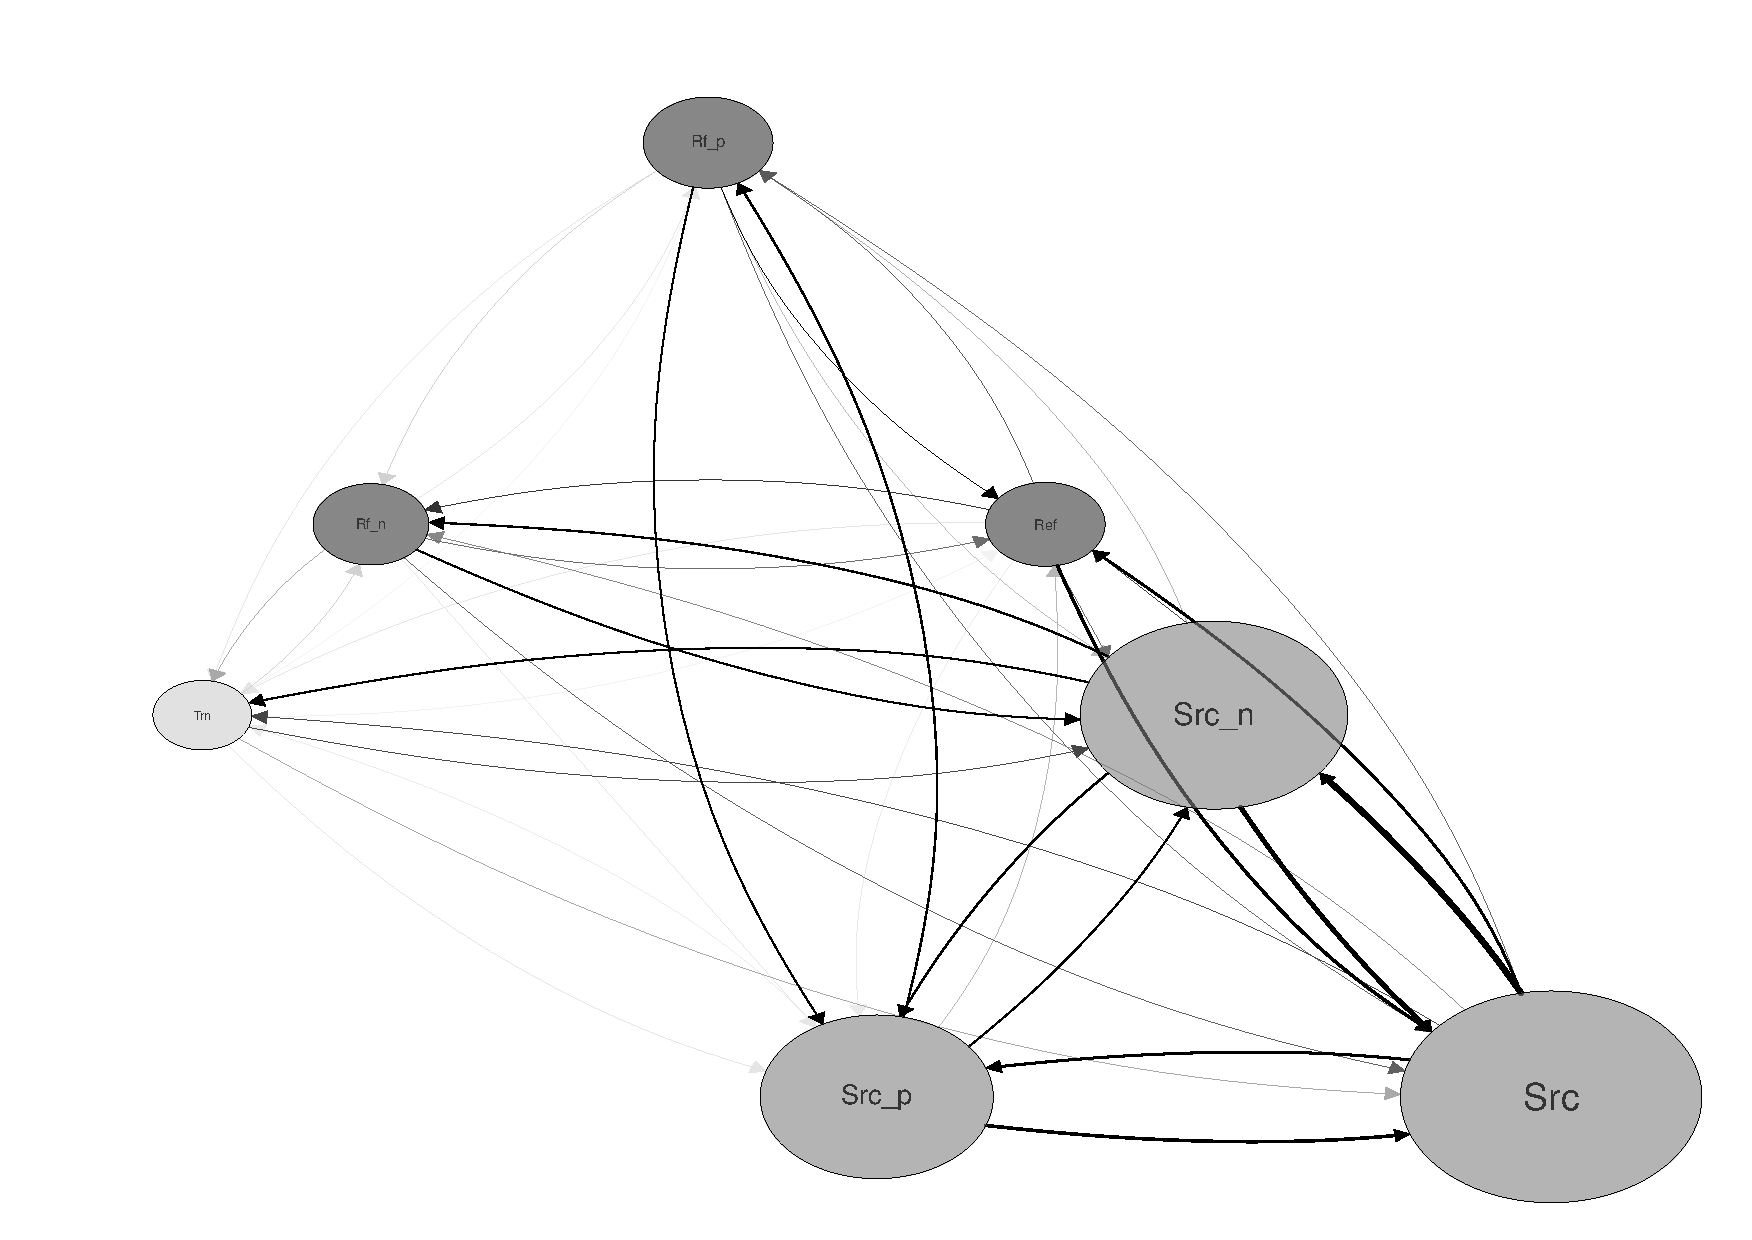
\includegraphics[scale=0.27]{data/behav_bilg_srctgt_max.pdf}
% \caption{Bilingual user process of scoring ``max'' category.}
% \label{fig:behavbilgmax}
% \end{figure}
% \begin{figure}[ht]
% \centering
% 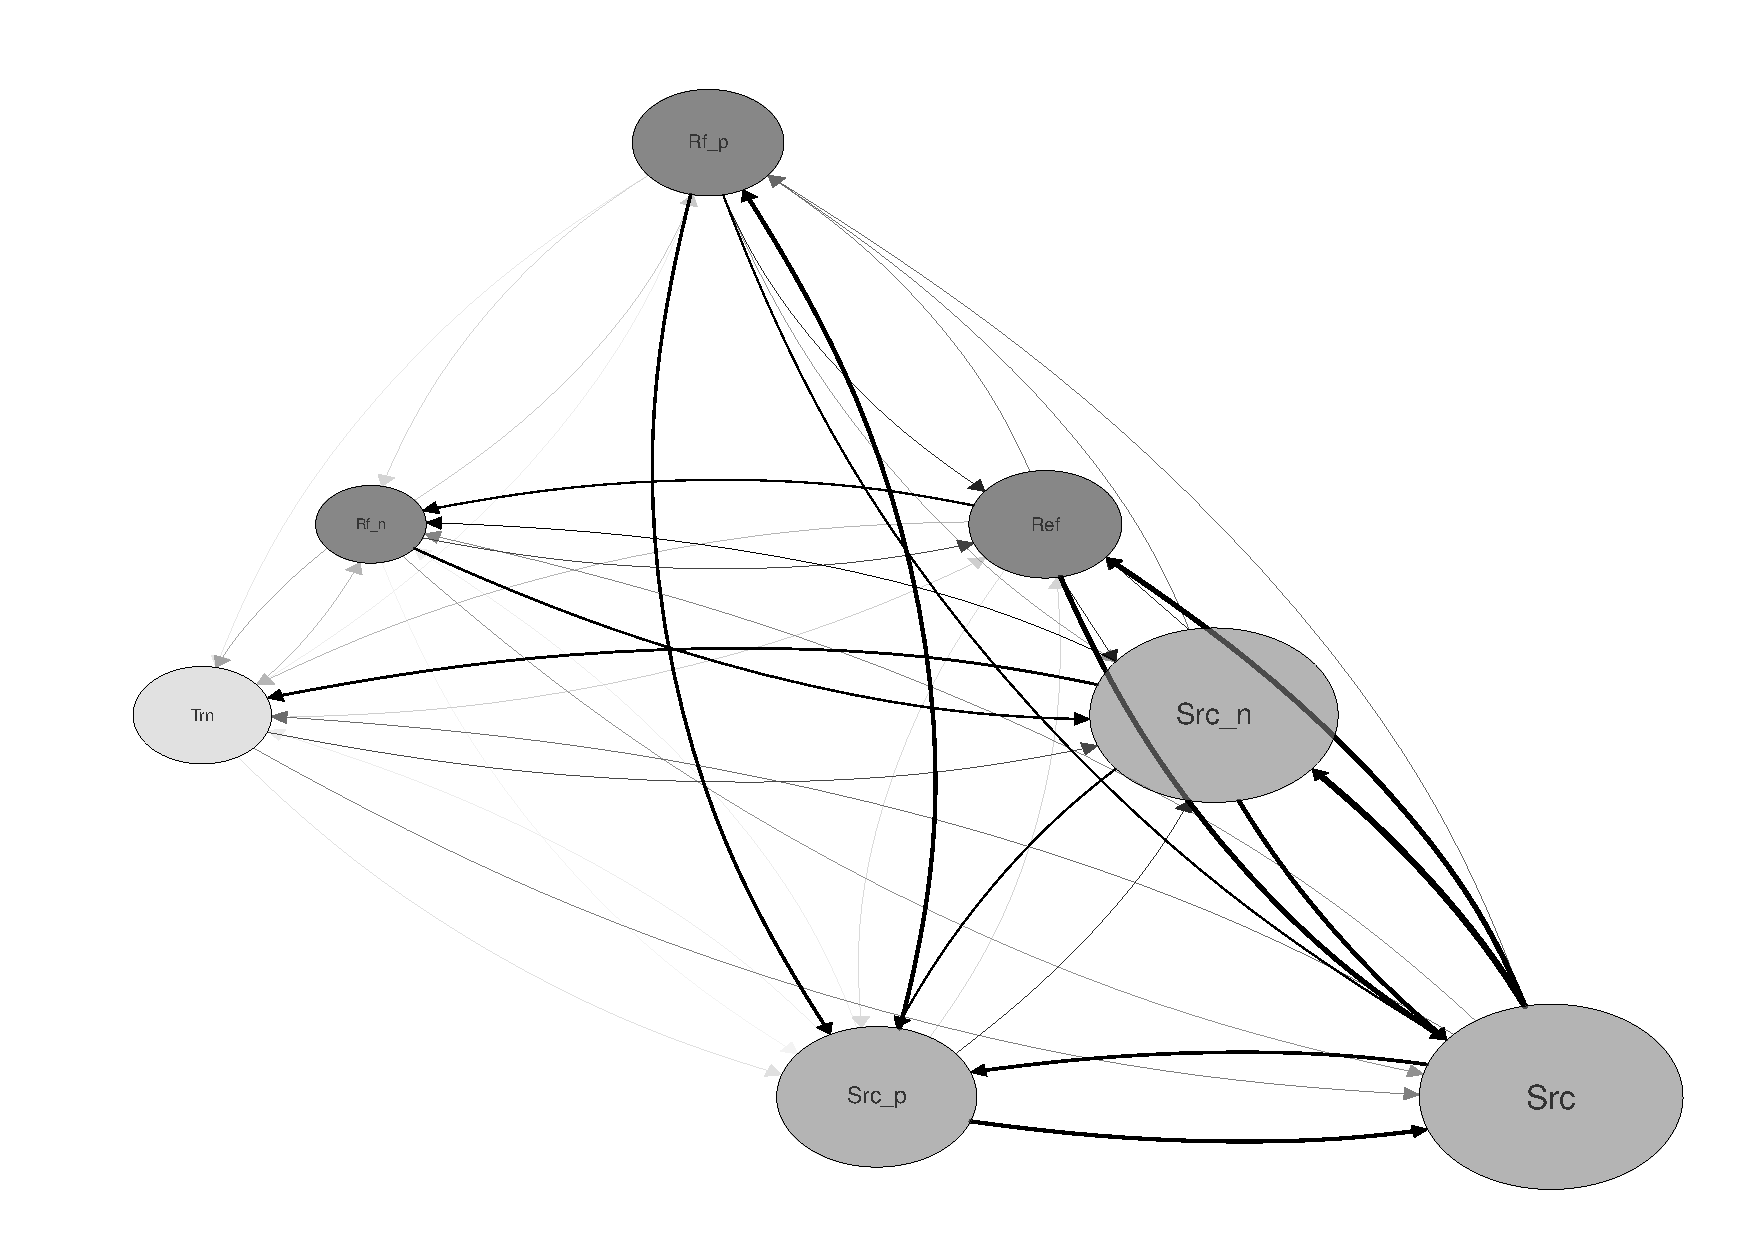
\includegraphics[scale=0.27]{data/behav_mono_srctgt_max.pdf}
% \caption{Monolingual user process of scoring ``max'' category.}
% \label{fig:behavmonomax}
% \end{figure}
% \\
%\if 0
% Conclusions:\\
% The results shows that while bilingual evaluators are typically faster that their monolingual peers, the latters are more consistent in their judgments. Monolingual inability to access source data, it is not an obstacle for them to make an accurate judgment.  On the other hand, when the hypotheses were scored with a language model. Monolingual looks like they are more consistent in mimicking language model scores as shown in Figure ~\ref{fig:costlm} -Dashed lines. 
% \begin{figure}[ht]
% \centering
% 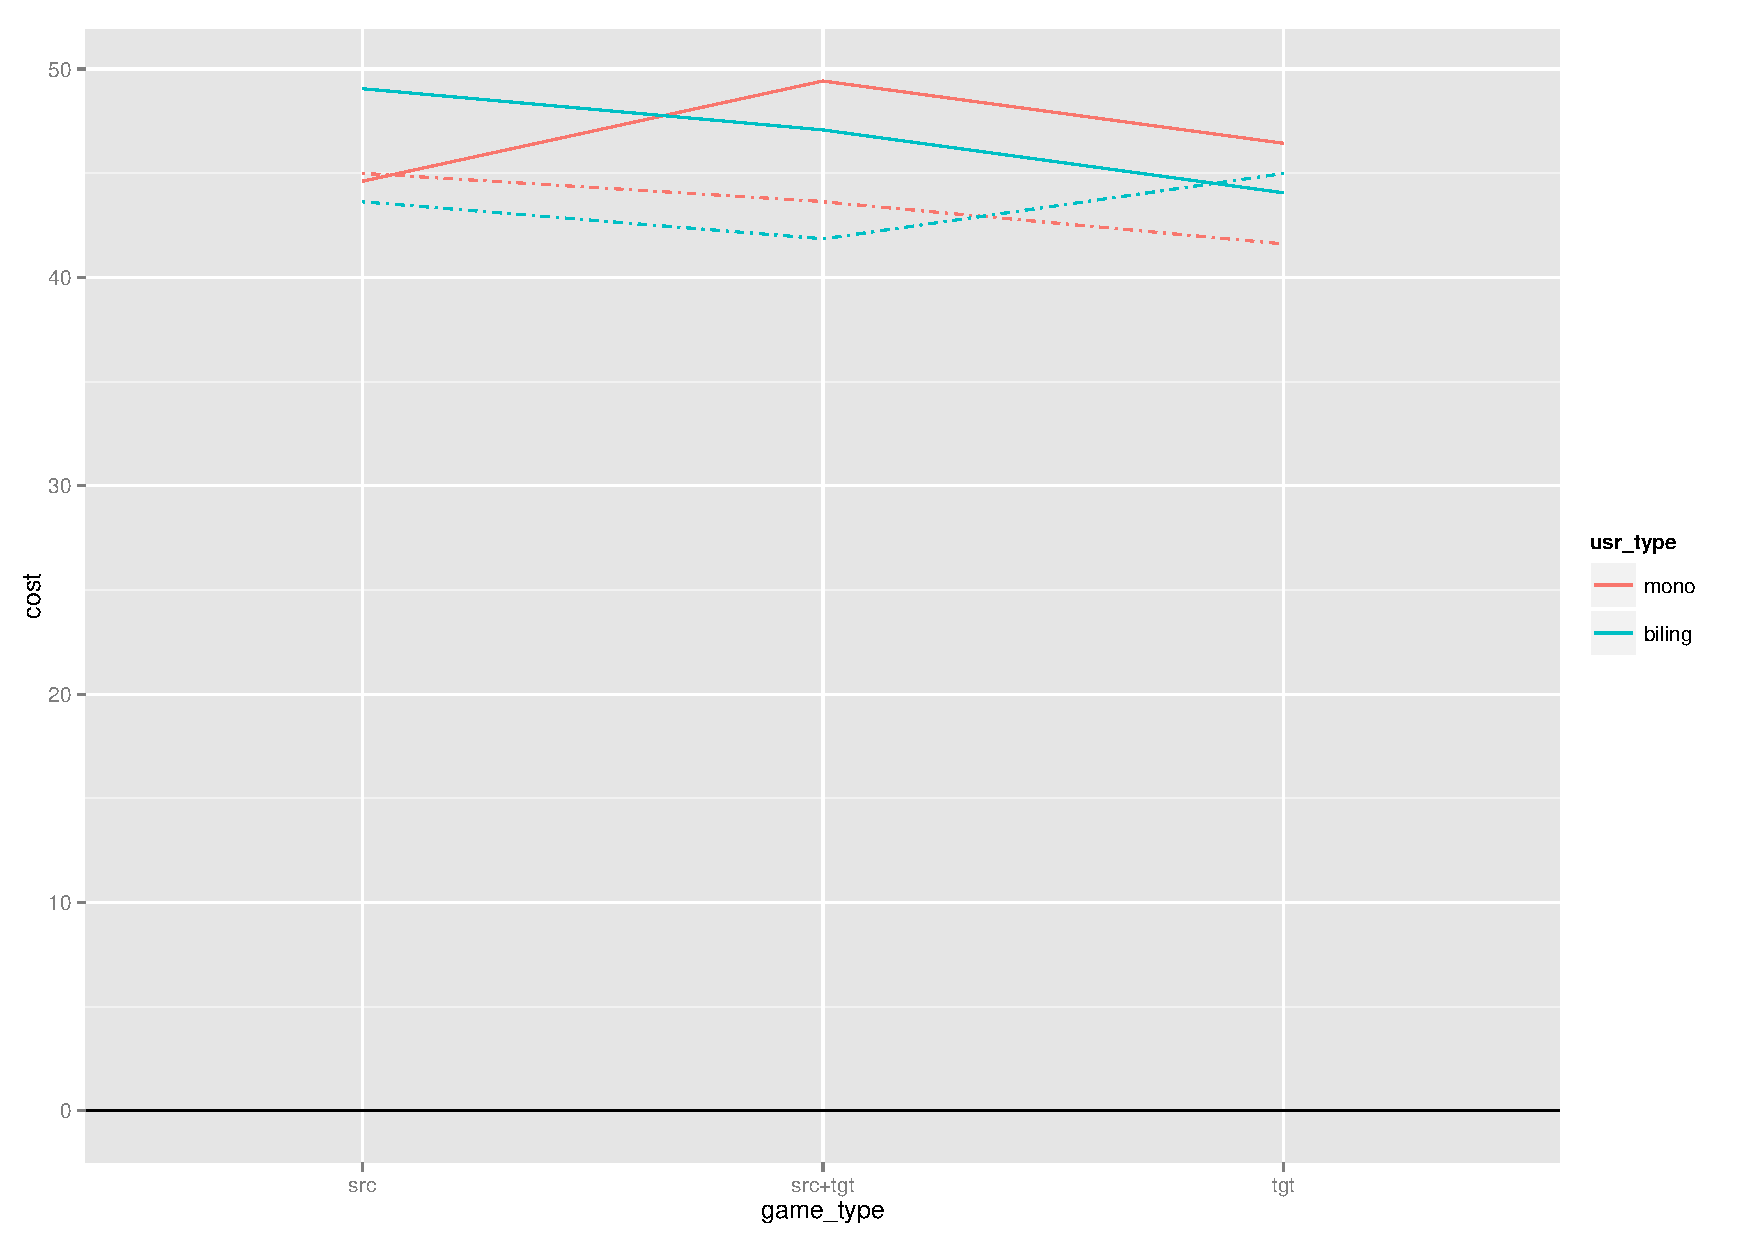
\includegraphics[scale=0.26]{data/cost_users_lm.pdf}
% \caption{Consistency of users vs humans and language model}
% \label{fig:costlm}
% \end{figure}
% %\fi

%So far, no huge difference between HIGH/LOW
